\chapter{Method} \label{cpt:method}
%This chapter should should include all the information required to make the study reproducible. 

\section{Introduction}

To gain familiarity with PINNs and explore their limitations, multiple PINNs were trained on data from different types of dynamical systems. The models were in some cases also compared against other models to highlight differences. After an initial investigation into how to work with PINNs, more advanced experiments were conducted that showcased more practical applications as well as better training methods.

All the PINN models were implemented from scratch with PyTorch \cite{pytorch} and functorch \cite{functorch}. The ODEs were integrated using torchdiffeq \cite{torchdiffeq}. The code is open sourced at \href{https://github.com/aljhn/master_project2}{{GitHub}}, using the MIT license for free use. The repository includes both code for training models as well as code for generating all the plots used throughout this thesis.

\section{Data}

The initial models were trained on generated synthetic data on relatively simple problems. The ODE systems were integrated using the Dormand-Prince 5 \cite{dopri} integrator with a step size of $h = 0.01$, where the initial values were both randomly sampled and manually chosen on different systems. The initial PDE systems were only using data generated from the initial and boundary conditions so it was not necessary to use a numerical solver. More data could be sampled from linear PDEs by solving them analytically using the separation of variables method. The analytical solution was also used for comparing the learned systems to the true systems as a form of training validation. Some experiments used datasets obtained from repositories associated with various papers. These datasets were used for validating the learned PINNs, and were originally obtained with traditional numerical solvers

The collocation points for calculating the physics informed loss were randomly sampled throughout the spatio-temporal domain. This can also be done when training PINNs on real data, as the collocation points do not rely on any information of the output of the system. The points were sampled uniformly as this turned out to work well enough instead of the latin hypercube sampling. Some of the simpler systems used linearly spaced collocation points instead of random sampling, but this proved to not be as effective for more complicated systems. More simpler PDEs could get away with sampling collocation points once before the training, while the more demanding PDEs sample collocation points randomly at every training iteration.

A manual seed was also set to ensure that the experiments were reproducible and to minimize the chance that the results are dependent on the random seed.

%\section{Data related information}
%How it was obtained/generated. Where can one find the data. 

%\section{Data pre-processing}
%How the data quality was improved for further analysis

\section{Model architecture}

The output trajectories of the dynamical systems were modeled as fully-connected neural networks. The $\tanh$ activation function was used to introduce nonlinearity and constrain the outputs of the hidden layers, while also allowing negative values. It is also continuously differentiable which could be an advantage when learning outputs that are also continuously differentiable. The physics informed loss was calculated using automatic differentiation to get first derivatives of the neural network at the collocation inputs, and second derivatives using the already calculated first derivatives as input to the automatic differentiation again. Higher order derivatives can be calculated in a similar manner.

When learning higher order ODEs with PINNs it is possible to convert the system dynamics into a state space representation and use that as the prior when computing the loss. This would however require collocation samples from a higher dimensional space, and potentially also more data corresponding to all the new states to accurately learn. For systems defined with a single state and higher order derivatives of that state it is then more useful to not use the state space representation as it is less data-intensive.

The MSE loss function was used for all purposes during training.

\section{Hyperparameters}

Table \ref{table:hyperparameters} contains a list of the hyperparameters for each of the conducted experiments. $\alpha$ refers to the learning rate, $N_u$ to the number of datapoints in the training set, $N_f$ to the number of collocation points and $\beta$ to the relative weighting of the loss functions. Each experiment is explained in more detail in the next section. Every experiment uses the Adam optimizer with some exceptions that use the L-BFGS optimizer, which can be seen in the table below when $\alpha = 1$. In general, it was found that the L-BFGS optimizer converges much faster, but is generally not practical for systems with more complicated dynamics where the optimizer can get stuck in a suboptimal minimum.

\begin{table}[H]
    \begin{adjustwidth}{-1cm}{-1cm}
    \caption{Table of hyperparameters for each experiment.}
    \begin{tabular}{ |c|c|c|c|c|c|c|c| }
        \hline
        Experiment & Hidden Layers & Hidden Units & Epochs & $\alpha$ & $N_u$ & $N_f$ & $\beta$ \\
        \hline
        \hline
        \multicolumn{8}{|c|}{\textbf{Learning Dynamical Systems with PINNs}} \\
        \hline
        \hline
        Linear ODE & 3 & 20 & 20000 & 1e-4 & 10 & 100 & 1e-4 \\
        \hline
        Nonlinear ODE & 4 & 20 & 10000 & 1e-4 & 10 & 100 & 1e-1 \\
        \hline
        Time-varying ODE & 2 & 40 & 1000 & 1e-3 & 1 & 1000 & 1e-1 \\
        \hline
        1D Linear PDE & 4 & 20 & 1000 & 1e-3 & 100 & 1000 & 1e-1 \\
        \hline
        2D Linear PDE & 4 & 20 & 1000 & 1e-3 & 100 & 1000 & 1e-3 \\
        \hline
        Nonlinear PDE & 5 & 20 & 1000 & 1 & 100 & 10000 & 1e-1 \\
        \hline
        \hline
        \multicolumn{8}{|c|}{\textbf{Data-Driven Discovery of Dynamical Systems with PINNs}} \\
        \hline
        \hline
        1D Linear PDE & 4 & 20 & 1000 & 1 & 1000 & 1000 & 1e-2 \\
        \hline
        2D Linear PDE & 4 & 20 & 1000 & 1 & 20000 & 20000 & 1e-4 \\
        \hline
        \hline
        \multicolumn{8}{|c|}{\textbf{Causal Training}} \\
        \hline
        \hline
        Simple PDE & 5 & 50 & 10000 & 1e-3 & 1000 & 10000 & 1e-3 \\
        \hline
        Chaotic PDE & 4 & 100 & 150000 & 1e-3 & 1000 & 25000 & 1e-3 \\
        \hline
        \hline
        \multicolumn{8}{|c|}{\textbf{Symbolic Operator Discovery}} \\
        \hline
        \hline
        Nonlinear PDE & 6 & 50 & 10000 & 1e-3 & 1000 & 10000 & 1e-3 \\
        \hline
        \hline
        \multicolumn{8}{|c|}{\textbf{Solving PDE-Constrained Optimal Control Problems with PINNs}} \\
        \hline
        \hline
        Flux Control & 5 & 50 & 5000 & 1 & 100 & 10000 & 100 \\
        \hline
        Dirichlet Boundary Control & 4 & 50 & 10000 & 1 & 100 & 10000 & 1 \\
        \hline
        Neumann Boundary Control & 4 & 50 & 10000 & 1 & 100 & 10000 & 1 \\
        \hline
        Initial Control & 4 & 50 & 20000 & 1e-3 & 400 & 20000 & 1 \\
        \hline
        \hline
        \multicolumn{8}{|c|}{\textbf{Regularization with the Maximum Principle}} \\
        \hline
        \hline
        Elliptic PDE & 4 & 50 & 1000 & 1 & 200 & 10000 & 1e-1 \\
        \hline
        \hline
        \multicolumn{8}{|c|}{\textbf{Causal Optimal Control with PINNs}} \\
        \hline
        \hline
        Initial Control & 5 & 50 & 20000 & 1e-3 & 1000 & 10000 & 1e4 \\
        \hline
        Reversed Initial Control & 5 & 50 & 20000 & 1e-3 & 1000 & 10000 & 1e3 \\
        \hline
    \end{tabular}
    \label{table:hyperparameters}
    \end{adjustwidth}
\end{table}

Some of the later experiments involve multiple neural networks being trained simultaneously. The listed hyperparameters in table \ref{table:hyperparameters} will in this case refer to the network that corresponds to the output state $u$. Other networks will usually have similar or slightly lower hidden layers and hidden units.

\section{Experimental Setup}

The following section describes the setup of each conducted experiment using the hyperparameters listed in table \ref{table:hyperparameters}. Details about the specific dynamical system along with parameters are described, in addition to what the purpose and goal of each experiment is. The results of each experiment are presented in the next chapter.

\subsection{Learning Dynamical Systems with PINNs}
\label{sec:method_learning_systems}

The first experiments are meant to show that PINNs can learn outputs from dynamical systems in a strictly superior way than standard neural networks by generalizing better on less data.

\subsubsection{Linear ODE}

Linear time-invariant ODEs are generally considered the easiest type of dynamical system to work with. They always have an analytical solution which can be expressed in a closed form, and are always stable or unstable on a global level. A common toy problem when working with ODEs is the second order dynamical system called the mass spring damper, which shows up in a variety of situations related to mechanical systems. The mass spring damper system is defined by the following ODE:

\begin{equation}
    m \ddot{x} + d \dot{x} + k x = 0
    \label{eq:msd}
\end{equation}

\noindent with state: position $x(t)$ and parameters: mass $m$, damping $d$ and spring constant $k$. The following experiments use the parameters: $m = 1, d = 5, k = 500$ and initial conditions $x(0) = 1, \dot{x}(0) = 0$.

\begin{figure}[H]
    \centering
    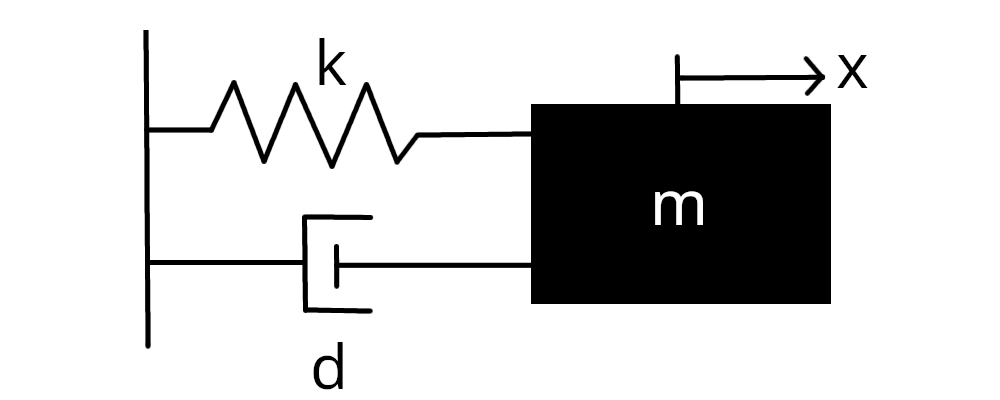
\includegraphics[width=0.8\linewidth]{Figures/Misc/massspringdamper.png}
    \caption{Mass spring damper system visualization.}
    \label{fig:massspringdamper}
\end{figure}

The purpose here is to demonstrate how to train PINNs on outputs from some of the simplest type of dynamical systems. A PINN is compared to a neural network with the same number of parameters trained in the standard way by formulating a regression problem on time inputs and trajectory outputs, to showcase the advantages of also incorporating prior information about the system dynamics. The training is done by sampling 10 datapoints evenly spaced in time in the range $0 < t < 0.4$ seconds from the true output of the system generated numerically. The training data only contains the positions $x(t)$ and not the velocity $\dot{x}(t)$. The mass spring damper is also used to demonstrate the importance of having enough data when training.

\subsubsection{Nonlinear ODE}

Consider the second order system called the Van der Pol oscillator defined by the nonlinear ODE:

\begin{equation}
    \ddot{x} - \mu (1 - x^2) \dot{x} + x = 0
    \label{eq:vdp}
\end{equation}

\noindent with state $x(t)$ and parameter $\mu$. It can be considered as a mass spring damper where $m = 1$, $d = - \mu (1 - x^2)$ and $k = 1$, and is a common example of an ODE with a limit cycle, meaning that every trajectory converges to some periodic function in time.

The parameter: $\mu$ is set to 1, and both a PINN and a standard neural network with the same number of parameters is trained on 10 datapoints evenly spaced throughout $0 < t < 20$. The purpose is to show that PINNs are able to easily generalize to nonlinear systems without losing any accuracy.

\subsubsection{Time-varying ODE}

For the final ODE, consider the non-autonomous Riccati equation defined by \cite{odebook}:

\begin{equation}
    \dot{x} = x^2 - t
    \label{eq:riccati}
\end{equation}

This system has two equilibrium points located at $x(t) = \pm \sqrt{t}$ where the negative equilibrium point is stable and the positive is unstable. This means that every initial condition below zero will approach the trajectory $x(t) = - \sqrt{t}$. This is demonstrated by training a PINN with equation (\ref{eq:riccati}) as prior but not using any datapoints at all. A second PINN is also trained by additionally using the initial condition as a datapoint.

\subsubsection{1D Linear PDE}

PINNs were originally formulated based on PDEs, as they are generally more difficult to work with than ODEs. The initial PDE experiment considered the 1-dimensional heat equation defined as follows:

\begin{equation}
    u_t = k^2 u_{xx}
    \label{eq:heat1d}
\end{equation}

The following experiment is defined by setting $k = 1$, boundary conditions $u(t, 0) = u(t, 1) = 0$ defined on the spatial region $0 < x < 1$ and initial condition $u(0, x) = \sin(\pi x)$. This makes it possible to solve the heat equation analytically using the separation of variables method. The initial condition was chosen strategically to simplify the computation of the resulting Fourier series from equation (\ref{eq:fourierpdecoeff}). The resulting solution has the expression:

\begin{equation}
    u(t, x) = \sin(\pi x) e^{- \pi^2 t}
    \label{eq:heat1dsolution}
\end{equation}

Figure \ref{fig:heat1d_true} displays a visualization of the state $u(t, x)$ over the spatial domain and the time range $0 < t < 0.2$ seconds, which is generated using the analytical expression (\ref{eq:heat1dsolution}). As the boundary is set to zero it will lead to an initial heat distribution evolving in time by dissipating towards zero.

\begin{figure}[H]
    \centering
    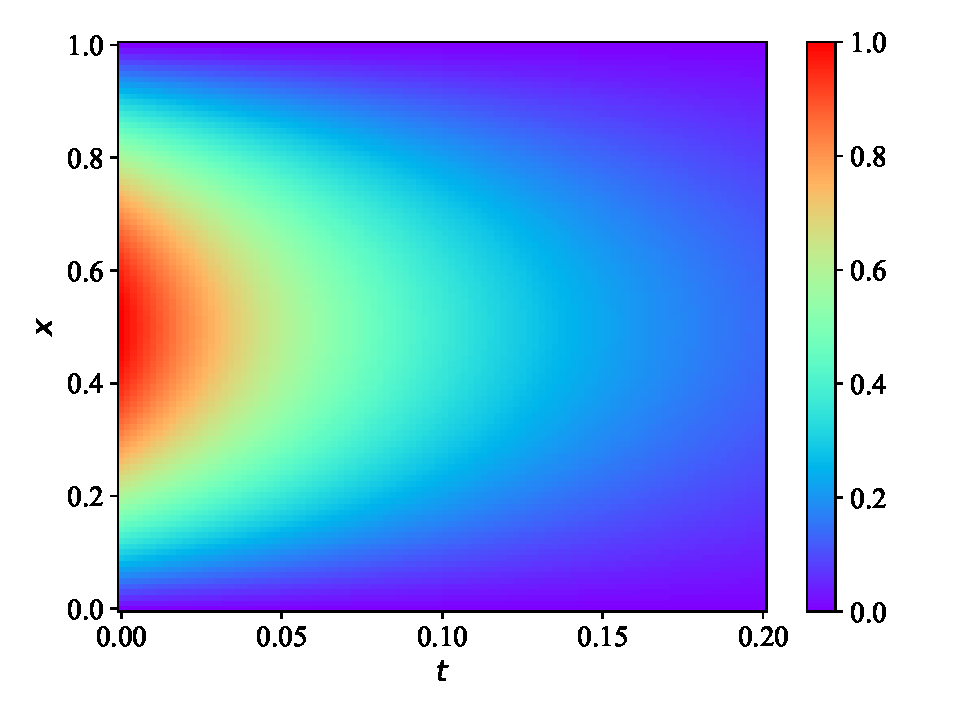
\includegraphics[width=1.0\linewidth]{Figures/InitialExperiments/heat1d_true.pdf}
    \caption{True solution of a 1-dimensional heat equation.}
    \label{fig:heat1d_true}
\end{figure}

Training a PINN is done by only using datapoints sampled randomly and uniformly on the boundary and initial conditions. Many real life problems modeled with PDEs have known expressions for the initial and boundary conditions which means that the current setup is equivalent to standard numerical solvers in terms of how much prior data they need. The collocation points for the physics informed loss are uniformly sampled across the whole spatio-temporal domain.

\subsubsection{2D Linear PDE}

Extending the previous experiment to the 2-dimensional heat equation defined as follows:

\begin{equation}
    u_t = k^2 (u_{xx} + u_{yy})
    \label{eq:heat2d}
\end{equation}

\noindent for spatial variables $x$ and $y$. The experiment uses a very similar setup where $k = 1$, the initial condition is given as: $u(0, x, y) = \sin(\pi x) \sin(\pi y)$ for $0 < x, y < 1$ and boundary conditions: $u(t, 0, y) = u(t, 1, y) = u(t, x, 0) = u(t, x, 1) = 0$. Similarly to the 1-dimensional case, an analytical solution can be found from the separation of variables method. This results in the expression:

\begin{equation}
    u(t, x, y) = \sin(\pi x) \sin(\pi y) e^{- 2 \pi^2 t}
    \label{eq:heat2dsolution}
\end{equation}

The true solution is visualized below in Figure \ref{fig:heat2d_true}. As the solution is three-dimensional it was visualized by extracting 2-dimensional slices in time to see how the spatial domain evolves.

\begin{figure}[H]
     \centering
     \begin{subfigure}[b]{0.45\textwidth}
         \centering
         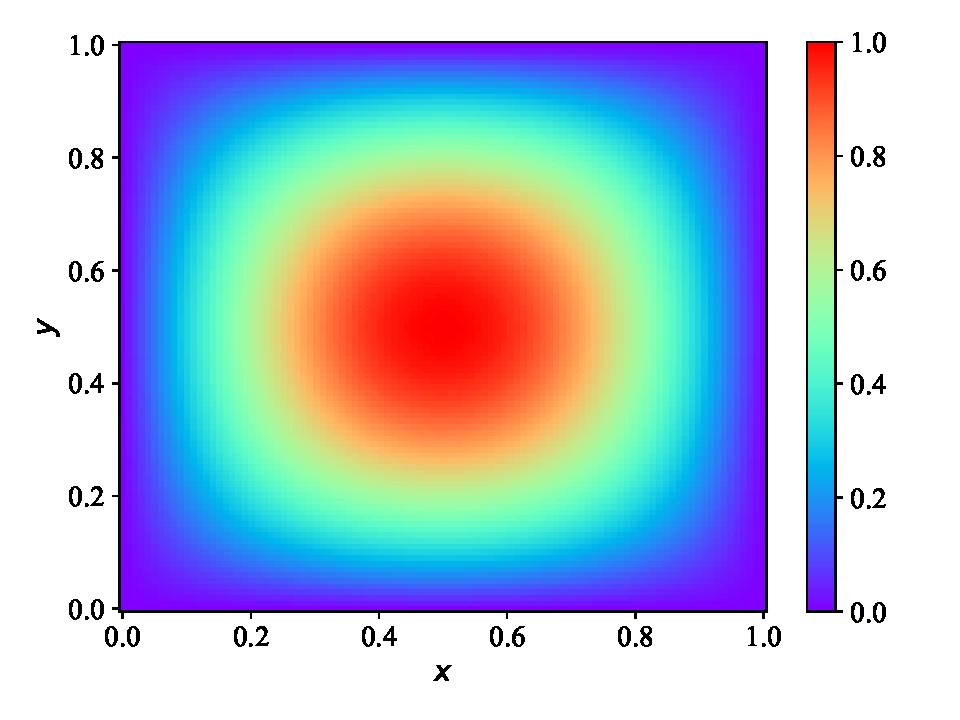
\includegraphics[width=\textwidth]{Figures/InitialExperiments/heat2d_1_true.pdf}
         \caption{$t = 0$}
         \label{fig:heat2d_1_true}
     \end{subfigure}
     \hfill
     \begin{subfigure}[b]{0.45\textwidth}
         \centering
         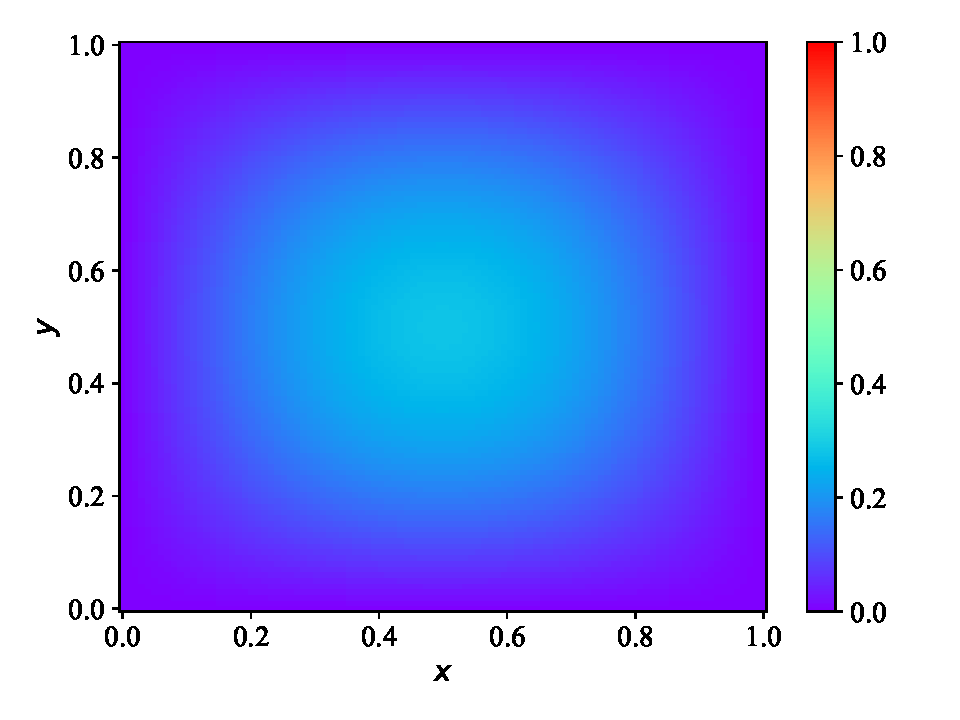
\includegraphics[width=\textwidth]{Figures/InitialExperiments/heat2d_2_true.pdf}
         \caption{$t = 0.067$}
         \label{fig:heat2d_2_true}
     \end{subfigure}
     \vskip\baselineskip
     \begin{subfigure}[b]{0.45\textwidth}
         \centering
         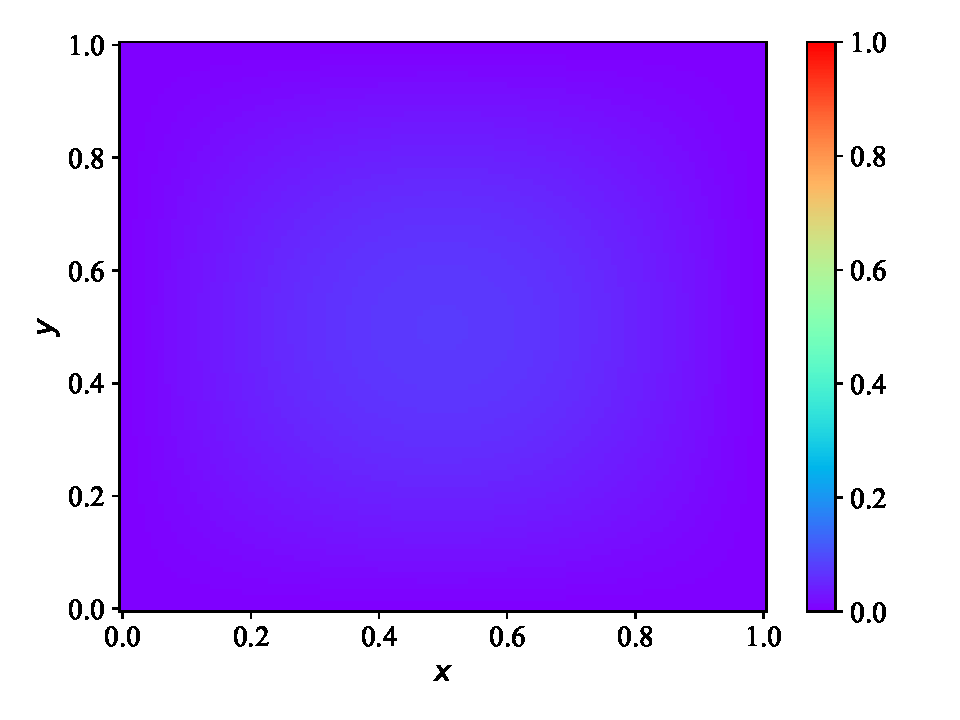
\includegraphics[width=\textwidth]{Figures/InitialExperiments/heat2d_3_true.pdf}
         \caption{$t = 0.133$}
         \label{fig:heat2d_3_true}
     \end{subfigure}
     \hfill
     \begin{subfigure}[b]{0.45\textwidth}
         \centering
         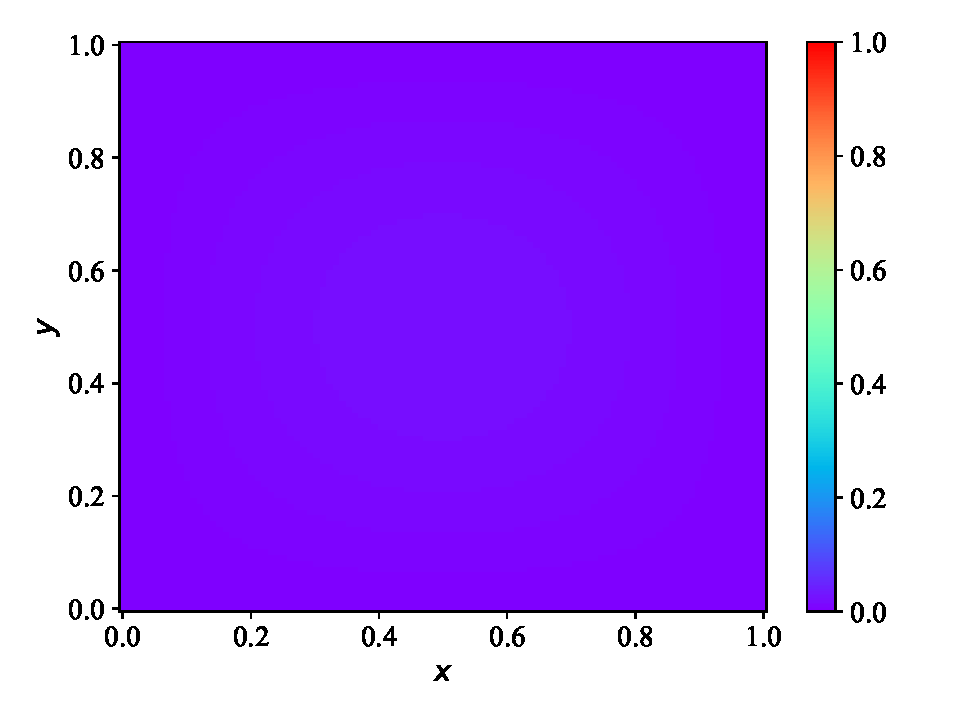
\includegraphics[width=\textwidth]{Figures/InitialExperiments/heat2d_4_true.pdf}
         \caption{$t = 0.2$}
         \label{fig:heat2d_4_true}
     \end{subfigure}
    \caption{True solution of a 2-dimensional heat equation.}
    \label{fig:heat2d_true}
\end{figure}

A PINN is trained with the exact same method as the previous 1-dimensional case by using uniformly sampled datapoints along the initial and boundary conditions for the regression loss and uniformly sampled collocation points. The goal of this experiment is to demonstrate that PINNs are able to learn higher dimensional PDEs, but with some more difficulty.

\subsubsection{Nonlinear PDE}

Nonlinear PDEs are usually not solvable analytically and can in many cases also be difficult to accurately solve numerically. The Navier-Stokes equations for describing fluid mechanics has an infamous open problem in mathematics regarding simply the existence of smooth solutions in 3-dimensional space. The homogeneous incompressible Navier-Stokes equations are defined as:

\begin{equation}
    \begin{cases}
        \bm{u}_t + (\bm{u} \cdot \nabla) \bm{u} - \nu \nabla^2 \bm{u} = - \frac{1}{\rho} \nabla p, & \\
        \nabla \cdot \bm{u} = 0, & 
    \end{cases}
\end{equation}

\noindent for states: velocity field $\bm{u}(t, \bm{x})$ and pressure $p(t, \bm{x})$, with parameters: viscosity $\nu$ and density $\rho$.

The viscous Burgers' equation can be derived from the Navier-Stokes equation by reducing to the 1-dimensional case, setting the pressure equal to zero and removing the constraint that the fluid flow is incompressible. This results in the following PDE:

\begin{equation}
    u_t + u u_x - \nu u_{xx} = 0
\end{equation}

The experiment uses the parameter $\nu = \frac{0.01}{\pi}$, initial condition $u(0, x) = - \sin(\pi x)$ and boundary conditions $u(t, -1) = u(t, 1) = 0$.

The Adam optimizer from the previous experiments are replaced with the L-BFGS optimizer using a line search based on the strong Wolfe conditions. It also requires significantly more collocation points to learn properly, but not any more datapoints along the initial and boundary conditions. The Burgers' equation is generally difficult to solve numerically due to a shock formation that forms after a certain amount of time \cite{pinn1}, but is still possible to learn with PINNs, although at an increased computational cost compared to simpler PDEs.

\subsection{Data-Driven Discovery of Dynamical Systems with PINNs}

The next set of experiments are meant to demonstrate an area where PINNs outperforms alternative numerical methods, as it can also be used with partially unknown dynamics. One of the advantages of machine learning compared to many classical alternatives is that the methods do not rely on an explicit model of the target system, which would have been subjected to potentially inaccurate assumptions and modeling errors. 

\subsubsection{1D Linear PDE}

The same heat equation problem formulated in the previous subsection is now revisited, except that the parameter $k$ is now considered unknown, thus leading to an incomplete model of the system dynamics. Using the approach described in \cite{pinn2} it is possible to train a PINN on data from the system and also learn an estimate of the $k$ parameter simultaneously. This is meant to be an experiment that showcases how the method works, which means it can also be applied to real data without knowing the analytical solution, or even the full details of the system dynamics.

The heat equation with the given setup was chosen for this experiment because it has a simple analytical solution that can be used to generate data and also verify the solution. The training data is now generated by random uniform sampling from the entire spatio-temporal domain, and the collocation points for the physics informed loss are chosen to be the same points as where the training data is collected. It therefore requires a lot more data than the case where the parameter is known. The L-BFGS optimizer is also used instead of Adam.

The estimated $\hat{k}$ parameter is randomly initialized by sampling from a standard normal distribution, and is then included as a part of the optimization procedure by augmenting it into the target vector. It is then optimized iteratively with L-BFGS using gradients computed from the physics informed loss function to the parameter $\hat{k}$ with automatic differentiation.

\subsubsection{2D Linear PDE}

To show that the data-driven discovery method can be applied to higher dimensional systems, the same experiment is now repeated for the 2-dimensional heat equation, also using the same setup as described in the previous subsection. The same changes are made to this experiment by using the L-BFGS optimizer, random uniform sampling of the same training and collocation points from the analytical solution, and initializing the estimated parameter $\hat{k}$ from a standard normal distribution. As the dimension is higher than the previous experiment, the number of training points has to be greatly increased to compensate.

\subsection{Causal Training}

This and the following subsections are meant to demonstrate more involved training methods and applications of PINNs. This subsection will demonstrate various enhanced techniques that can be applied during training to improve accuracy and robustness, in some cases also convergence speed. This also makes it possible to solve PDEs that standard PINNs have historically failed to properly learn, like certain chaotic systems.

These experiments are meant to demonstrate the theory outlined in the literature review from the previous chapter.

\subsubsection{Simple PDE}

Once again, consider the Burgers' equation defined as:

\begin{equation}
    u_t + u u_x - \nu u_{xx} = 0
\end{equation}

\noindent with the parameter $\nu = \frac{0.01}{\pi}$, initial condition $u(0, x) = - \sin(\pi x)$ and periodic boundary conditions $u(t, -1) = u(t, 1) = 0$.

The purpose now is to demonstrate \ref{sec:method_learning_systems} how the learned solution can be improved from the previous experiment. Because the boundary conditions are defined to be periodic, this is enforced exactly using a Fourier embedding. The Fourier embedding uses 5 increasing frequencies of sines and cosines in addition to the DC-term, which means that the spatial input dimension of the network becomes 11, in addition to one extra time dimension. Because all the frequencies are set to be periodic on the boundary, the periodic boundary conditions are satisfied automatically without adding any extra boundary term to the loss function.

The neural network itself is implemented as the modified network structure with residual connections, which has been shown to improve gradient flow for many chaotic systems.

This is combined with the causal loss function (\ref{eq:causal_loss}) which prioritizes learning earlier time-domains before later time-domains, ensuring that causality in time is prioritized during training. The causal loss is created by dividing the time domain into 20 equally sized subdomains.

The full training procedure, each running a certain amount of epochs, is done for 5 different values of the $\epsilon$ hyperparameter. $\epsilon$ is first initialized to $0.01$, and training is either done until max epochs is reached, or a convergence criterion depending on the loss weightings are met. $\epsilon$ is then multiplied by $10$ for each subsequent training run, ending with a value of $100$ for the final iteration. This makes it so that causality is enforced more for later training runs compared to the first ones. Each training run continues with the same network parameters from the previous run, thus each subsequent run can be thought of as an additional fine-tune that makes everything gradually more causal.

The final enhancement is to add time-marching. The overall time domain is split into 10 different equally sized subdomains, and a separate model is trained on each subdomain. This also means that each of these 10 subdomains are further divided into 20 subdomains from the causal loss. When one network finishes training, the next network is initialized with the parameters of the previous network before restarting on the next time subdomain. This also means that to get the output solution for the whole domain, the outputs of each submodel must be combined together.

\subsubsection{Chaotic PDE}

Burgers' equation was already possible to solve accurately without the causal enhancements, so the vastly increased training time is not necessarily justified. The previous experiment was meant to show that the new techniques actually work, before attempting a more complicated equation.

Now consider the 1-dimensional Allen-Cahn equation defined as:

\begin{equation}
    u_t - 0.0001u_{xx} + 5 u^3 - 5 u = 0
\end{equation}

\noindent on the domain $0 \leq t \leq 1$ and $-1 \leq x \leq 1$, using initial condition: $u(0, x) = x^2 \cos(\pi x)$ and periodic boundary conditions: $u(t, -1) = u(t, 1)$ and $u_x(t, -1) = u_x(t, 1)$.

This is an example of a chaotic PDE where standard PINNs fail to properly learn the true solution, causing the error between the true solution and the PINN solution to increase along the time axis.

Training a PINN with the same enhanced training techniques as used for the Burger's equation in the previous experiment makes it possible to accurately learn the Allen-Cahn equation. A modified network structure is used alongside Fourier embeddings, this time using 10 increasing frequencies resulting in an input dimension of 22. The causal loss is subdivided into 100 time-domains. Time-marching is not used, as this is one of the more computationally demanding techniques, and is instead replaced with more collocation points and network parameters to compensate. The $\epsilon$ hyperparameter is set to the constant $100$ instead of iterating through a list.

To verify the accuracy of the solution, the trained PINN is compared to a dataset obtained from a traditional numerical solver \cite{pinncausalitygithub}.

\subsection{Symbolic Operator Discovery}

The previous subsection on data-driven discovery of PDEs demonstrated a use case of PINNs where they perform better than traditional numerical solvers. In that case, the dynamics of the system was known in the form of the full PDE, with the addition that there are unknown parameters to be learned in addition to the full solution.

Full system equations can in many cases be explicitly derived from first principles, which makes the previous experiment useful in many cases. However, when using first principles there are always many assumptions and simplifications being made to make it possible to model the true system. In some cases, this can lead to a model that is not accurate enough to be useful for a given purpose. It is also possible that an equation is derived explicitly, but that some terms of the equation are missing.

The purpose of the following experiment is to make it possible to use data to discover new dynamics and possibly unknown terms of an equation. The symbolic operator discovery method described in the literature review is here used to learn a missing term of a PDE from data.

\subsubsection{Nonlinear PDE}

Burgers' equation is used yet again to demonstrate the method. Burgers' equation is now assumed to be on the form:

\begin{equation}
    u_t - \nu u_{xx} = 0
\end{equation}

\noindent with $\nu = \frac{0.01}{\pi}$ and where the term $u u_x$ is missing from the equation. The goal is to re-learn this term from data. The initial condition is set to the usual $u(0, x) = - \sin(\pi x)$ and boundary conditions are assumed to be periodic.

Because the boundary is assumed to be known explicitly, it is not necessary to use a dedicated network to learn this. The solution network and the unknown dynamics network are both set to standard neural networks with the same number of layers and hidden units, and then trained together. The unknown dynamics has an input dimension of 3, corresponding to the terms: $u$, $u_t$ and $u_x$. The true term is equal to the product of $u$ and $u_x$, meaning that $u_t$ is not actually needed. It is added as an input here, because in real applications it is not known beforehand which terms that goes in the unknown dynamics.

To verify the accuracy of the experiment, a separate PINN is trained on the Burgers' equation using all the same enhanced training techniques described in the previous subsection on causal training, except time-marching to make it easier to compare. The output of this PINN is then compared against a dataset obtained from a traditional numerical solver \cite{og_pinn_github}. For simplicity, this PINN is then used as the ground truth for comparing the learned dynamics in this experiment.

\subsection{Solving PDE-Constrained Optimal Control Problems}

The next set of experiments are meant to demonstrate a practical application of PINNs, and show that the same framework can solve many different types of problems. However, one drawback with this approach compared to traditional numerical methods is that there are fewer guarantees with regards to optimality of solutions and general accuracy of the solutions.

\subsubsection{Flux Control}

For the first experiment, consider a system governed by the two-dimensional Laplace equation:

\begin{equation}
    \frac{\partial^2 u}{\partial x^2} + \frac{\partial^2 u}{\partial y^2} = 0
\end{equation}

\noindent defined on the square domain: $(x, y) \in [0, 1] \times [0, 1]$, with boundary conditions:

\begin{itemize}
    \item $u(x, 0) = \sin (\pi x)$
    \item $u(x, 1) = c(x)$
    \item $u(0, y) = u(1, y)$
    \item $\frac{\partial u}{\partial x}(0, y) = \frac{\partial u}{\partial x}(1, y)$
\end{itemize}

\noindent with a periodic boundary in the x-direction, and where the function $c(x)$ is a control input that affects the entire top side of the domain.

Now consider the optimal control problem with all the above equations as constraints along with the objective function:

\begin{equation}
    J = \int_ {0}^{1} \begin{bmatrix} \frac{\partial u}{\partial y}(x, 1) - q_d(x) \end{bmatrix}^2 dx
\end{equation}

\noindent where $q_d(x) = \cos (\pi x)$ is the desired flux. The optimal control problem can be thought of as finding the control input $c(x)$ that results in the desired flux at the top side of the boundary, subject to the dynamics and boundary conditions.

The problem is solved using the method outlined in \cite{pinnoptimalcontrol}. Two neural networks are trained simultaneously, the first represents the state $u$ and the second represents the control input $c(x)$. The final loss function to be optimized is a weighted sum of the boundary loss, physics loss and objective function. The integral for the objective function is computed numerically using the trapezoid method of integration using 41 point evaluations along the integral. For this experiment, the weightings of the boundary and physics loss are set to be $1$, with a weighting of the objective function set to $100$.

\subsubsection{Dirichlet Boundary Control}

For this next experiment consider the optimal control problem with dynamics governed by the 1-dimensional heat equation:

\begin{equation}
    \frac{\partial u}{\partial t} - \frac{\partial^2 u}{\partial x^2} = 0
\end{equation}

\noindent with initial condition:

\begin{equation}
    u(0, x) = \sin (\pi x)
\end{equation}

\noindent and boundary condition:

\begin{equation}
    u(t, 0) = c(t)
\end{equation}

\noindent for a control input $c(t)$. This means that the control input can influence the dynamics along the bottom boundary of the domain. The objective function is here defined to be:

\begin{equation}
    J = \sum_{k=1}^{N} \begin{bmatrix} u(x_k) - u_d(x_k) \end{bmatrix}^2
\end{equation}

\noindent for a desired temperature distribution $u_d(x) = 0.5$. The objective function could be replaced with an integral and computed with the trapezoid method, similarly to the previous experiment. However, simply evaluating the function at a set of points and comparing these with the MSE loss works well enough. The objective function is evaluated at the final time of the temporal domain. This makes it so the system does not necessarily have to approach the target distribution as fast or as energy efficient as possible, which are usually desirable properties of control systems, but could also make the learning procedure more difficult as the the three losses are summed together.

\subsubsection{Neumann Boundary Control}

Now consider the same experiment as above, except that the boundary condition is given as:

\begin{equation}
    \frac{\partial u}{\partial x}(t, 0) = c(t)
\end{equation}

\noindent which is usually a more realistic scenario, as influencing the temperature distribution directly without any inertia is more difficult to do than setting the flux along the boundary.

\subsubsection{Initial Control}

For the final experiment here, consider the system governed by Burgers' equation:

\begin{equation}
    \frac{\partial u}{\partial t} + u \frac{\partial u}{\partial x} = \nu \frac{\partial^2 u}{\partial x^2}
\end{equation}

\noindent with $\nu = 0.01$. The domain is set to be $(t, x) \in [0, 5] \times [0, 4]$. Periodic boundary conditions are used.

It can be verified that the following analytical solution satisfies Burgers' equation \cite{pinnoptimalcontrol}:

\begin{equation}
    u_a(t, x) = \frac{2 \nu \pi e^{- \pi^2 \nu (t - 5)} \sin (\pi x)}{2 + e^{- \pi^2 \nu (t - 5)} \cos(\pi x)}
\end{equation}

\noindent so that the initial condition can be inferred to be: $u(0, x) = u_a(0, x)$. This analytical solution is visualized in Figure \ref{fig:burger_control_analytical}.

\begin{figure}[H]
    \centering
    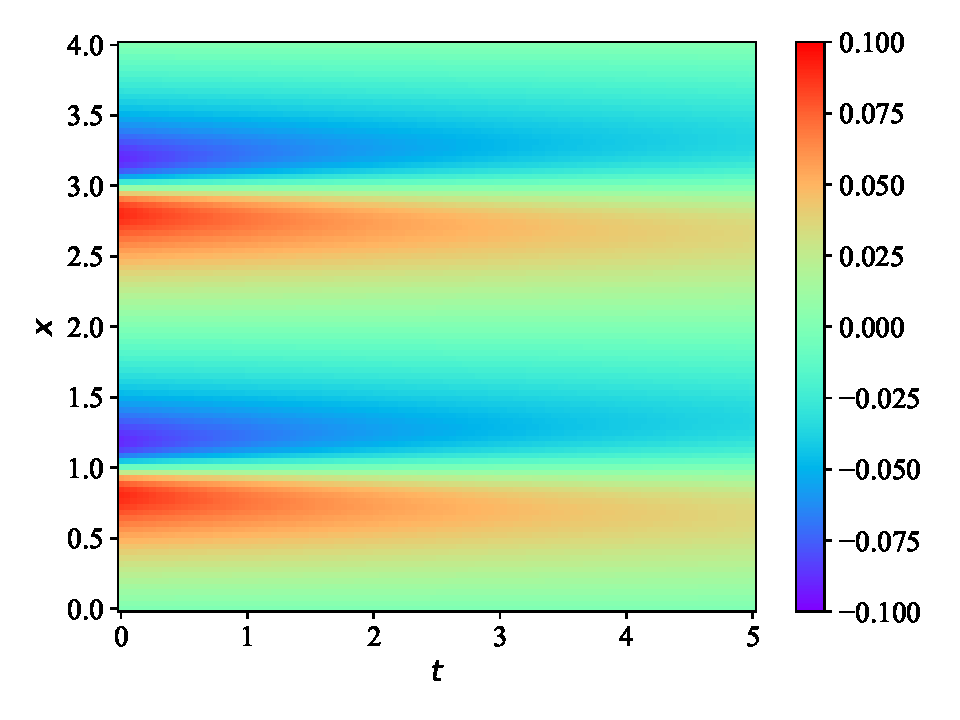
\includegraphics[width=1.0\linewidth]{Figures/IntermediateExperiments/OptimalControl/burger_control_true.pdf}
    \caption{An analytical solution of Burgers' equation.}
    \label{fig:burger_control_analytical}
\end{figure}

Now consider the optimal control problem by setting the initial condition to:

\begin{equation}
    u(0, x) = c(x)
\end{equation}

\noindent with control input c(x). The objective function is set to be:

\begin{equation}
    J = \frac{1}{2} \int_{0}^{4} \begin{bmatrix} u(5, x) - u_a(5, x) \end{bmatrix}^2 dx
\end{equation}

This means that the goal of the optimal control problem is to find the initial condition that results in the final state defined by $u_a(5, x)$. As solutions are unique, this implies that the resulting solution to the overall control problem will also equal $u_a(t, x)$ on the entirety of the domain.

The integral of the objective function is again computed numerically using trapezoid integration with 41 point evaluations.

\subsection{Regularization with the Maximum Principle}

The following experiment is based on a novel idea from this master project. It is a way to make the training loss converge faster, as well as make it possible to use fewer collocation points, which overall results in faster PINN training.

\subsubsection{Elliptic PDE}

A function is called harmonic if it satisfies Laplace's equation:

\begin{equation}
    \nabla^2 u = 0
\end{equation}

A function is called subharmonic if it satisfies the following inequality:

\begin{equation}
    \nabla^2 u \geq 0
\end{equation}

\noindent and the opposite inequality results in a superharmonic function. Harmonic functions are therefore both subharmonic and superharmonic \cite{pdebookcourse}.

For a subharmonic function $u$ defined on a bounded domain $\Omega \subset \mathbb{R}^n$, the strong maximum principle says that:

\begin{equation}
    \max_{\overline{\Omega}} u = \max_{\partial \Omega} u
\end{equation}

\noindent which either means that the maximum value of $u$ is attained at the boundary of the domain, or that $u$ is constant on the domain \cite{pdebookcourse}. This can be thought of as analogous as to how convex functions have their maximum values on the boundary of their domain, as long as the domain is also convex.

Similarly for superharmonic functions:

\begin{equation}
    \min_{\overline{\Omega}} u = \min_{\partial \Omega} u
\end{equation}

\noindent which also means that for a harmonic function $u$:

\begin{equation}
    \min_{\partial \Omega} u \leq u \leq \max_{\partial \Omega} u
\end{equation}

\noindent meaning that both the maximum and minimum values are attained at the boundary of the domain.

This can be used during PINN training by adding regularization terms to the loss function. The maximum regularization term can be computed by first finding the maximum value along the boundary:

\begin{equation}
    u_{\texttt{max}} = \max_{\partial \Omega} u
\end{equation}

\noindent and then penalizing values of $u$ that are above the max value on interior points:

\begin{equation}
    \mathcal{L}_{r^+} = \sum_{i=1}^{N_f} \begin{bmatrix} \max(u(t_f^i, x_f^i) - u_{\texttt{max}}, 0) \end{bmatrix}^2
\end{equation}

\noindent using the same collocation points $(t_f^i, x_f^i)$ as the physics informed loss. If $u(t_f^i, x_f^i) - u_{\texttt{max}} > 0$ for any interior point, this is added to the regularization sum. If it is smaller than zero, it is set to 0 from the $\max$ statement and therefore not added to the regularization. The max value is also computed again for every training iteration. If the boundary conditions are known explicitly, it could be possible to use a constant max value computed from this.

The minimum regularization is done similarly by first computing the minimum value on the boundary:

\begin{equation}
    u_{\texttt{min}} = \min_{\partial \Omega} u
\end{equation}

\noindent and then summing up points:

\begin{equation}
    \mathcal{L}_{r^-} = \sum_{i=1}^{N_f} \begin{bmatrix} \min(u(t_f^i, x_f^i) - u_{\texttt{min}}, 0) \end{bmatrix}^2
\end{equation}

Both maximum and minimum regularization use values raised to the second power. For the minimum regularization, this serves as a way to make the values positive, but the maximum values are always positive. Raising to the second power is also differentiable, unlike the alternative solution of using an absolute value for the minimum. This can also be thought of as similar to how L1 versus L2 regularization on network parameters leads to different outcomes. L1 regularization tends to drive the parameters closer to zero, while L2 places less importance on smaller values and more on removing the big outliers.

Combining the maximum and minimum regularization terms leads to the overall regularization:

\begin{equation}
    \mathcal{L}_r = \mathcal{L}_{r^+} + \mathcal{L}_{r^-}
    \label{eq:maxminreg}
\end{equation}

To test the effectiveness of this new regularization term, consider Laplace's equation in two dimensions and the following analytical solution:

\begin{equation}
    u_a(x, y) = \cos(\pi x) \sinh (\pi y)
\end{equation}

\noindent defined on the domain $(x, y) \in [0, 1] \times [0, 1]$. The analytical solution can be derived using separation of variables and is easily verifiable to satisfy the equation. It is visualized in Figure \ref{fig:laplace_analytical}. This analytical solution can then be used to obtain boundary conditions and verify the accuracy of the trained PINNs.

\begin{figure}[H]
    \centering
    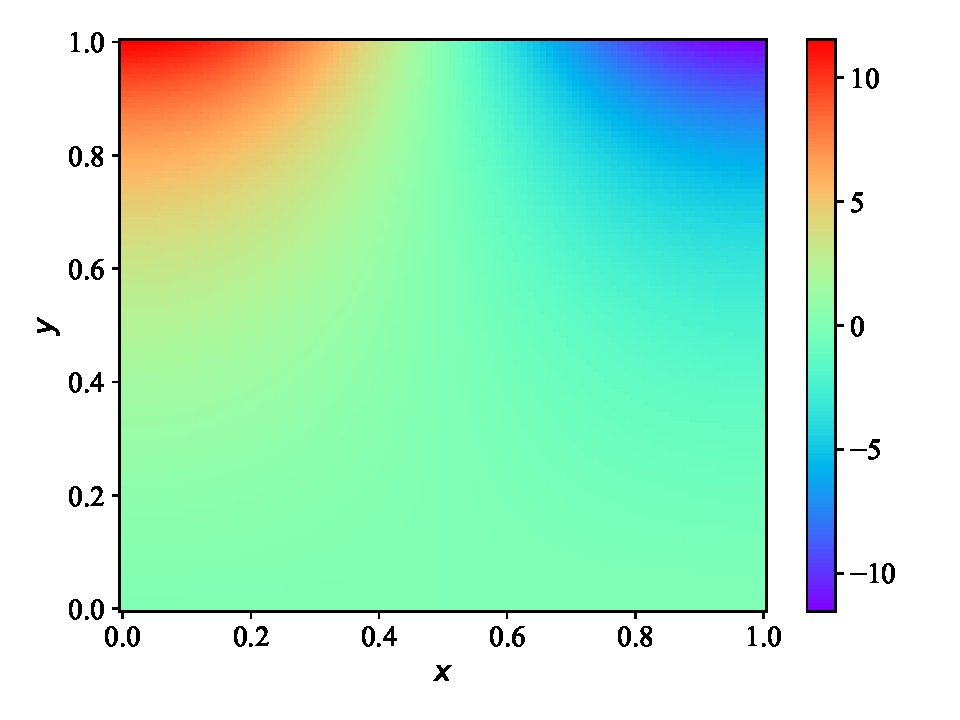
\includegraphics[width=1.0\linewidth]{Figures/IntermediateExperiments/Laplace/laplace_forward_true.pdf}
    \caption{An analytical solution of Laplace's equation.}
    \label{fig:laplace_analytical}
\end{figure}

Two PINNs with the same number of parameters are trained independently of each other on Laplace's equation with boundary conditions obtained from the analytical solution. One of the PINNs is trained with the standard PINN setup, while the other one has the exact same setup and hyperparameters with the addition of the regularization term (\ref{eq:maxminreg}).

Afterwards, both PINNs are trained again from scratch, only this time using much less collocation points with a reduction from 10000 to 200.

For PDEs that are more complicated than Laplace's equation, it is also possible to generalize a weaker version of the maximum principle. This requires that the PDE is uniformly elliptic. For a second order linear differential operator $L$, defined as:

\begin{equation}
    L = - \sum_{i=1}^{n} \sum_{j=1}^{n} a_{ij}(\bm{x}) \frac{\partial^2}{\partial x_i \partial x_j} + \sum_{j=1}^{n} b_j(\bm{x}) \frac{\partial}{\partial x_j}
\end{equation}

\noindent then, $L$ is elliptic if the eigenvalues of the matrix $\begin{bmatrix} a_{ij} \end{bmatrix}$ are positive at each point $\bm{x}$, and $L$ is uniformly positive if the smallest eigenvalue is bounded from below by a constant $\kappa > 0$ at each point $\bm{x}$. The difference between elliptic and uniformly elliptic is not that important for practical and numerical applications, and is mostly a necessity of mathematical rigor. So the maximum principle could be used for many different types of elliptic PDEs if they satisfy the above requirement.

Also note that the maximum principle for elliptic PDEs is unrelated to the similar sounding Pontryagin's maximum principle \cite{pontryagin62} from optimal control theory.

Finally, it should be mentioned that a similar maximum statement can be said about the heat equation, where the maximum value is attained either at the boundary of the domain, or at the initial time \cite{pdebookcourse}. Using this for faster training is less obvious to implement, and could be worth investigating further.

\subsection{Causal Optimal Control}

The final set of experiments use a combination of previous methods for an overall improvement. More specifically, the PINN approach to optimal control theory is combined with causality and related techniques to improve upon the training method.

\subsubsection{Initial Control}

The same initial control problem described above in the subection on optimal control theory is now re-visited with all the same improvements done when training on the chaotic PDE in the subsection on causal training. Causality leads to a more robust training in general, which should also be helpful in order to learn control policies more accurately.

\subsubsection{Reversed Initial Control}

For the problem with initial control, it might not necessarily make the most sense to apply causality forwards in time. This is because the initial condition is unknown while the final end state is known. So applying causality on an imperfect initial condition can in this case lead to a loss function with two terms that are competing against each other for most of the training. The term related to the causal physics information is trying to keep the initial condition accurate before moving on to the next time range. While the term related to the objective function of the optimal control problem wants to change the initial condition to fit the final end state, thus breaking the causal training.

A solution to this problem can be to re-formulate it by reversing the direction of the time $t$, and setting the desired final state as the initial condition. This also means that there is no longer any need for an explicit control policy, so this particular optimal control problem can be learned simply by causal training on the reversed time. The control policy corresponding to the initial condition for the actual problem then becomes equal to the end state of the reversed-time problem.

As the time range goes from $t = 0$ to $t = 5$, define the new reversed time variable as: $\tau = 5 - t$. By setting the state as a function: $u = u(\tau, x)$, then the partial derivative becomes:

\begin{equation}
    \frac{\partial u}{\partial t} = \frac{\partial u}{\partial \tau} \frac{\partial \tau}{\partial t} = - \frac{\partial u}{\partial \tau}
\end{equation}

The partial derivative for the spatial variable $x$ remains unchanged. The time-reversed Burgers' equation then becomes:

\begin{equation}
    - \frac{\partial u}{\partial \tau} + u \frac{\partial u}{\partial x} = \nu \frac{\partial^2 u}{\partial x^2}
\end{equation}

\noindent which can now be used instead of the forward-time version of the equation for the physics informed loss.

%\section{Scenario and case set-up}

%Present the information in tables and figures. 
